\section*{Results and Discussion}

%%%%%%%%%%%%%%%%%%%%%%%%%%%%%%%%%%%%%%%%%%%%%%%%%%%%%%%%%%%%
\renewcommand{\arraystretch}{1.1}
\begin{table}[tb]

\begin{center}
 \caption[]{Silent site $F_{ST}$ from GBS SNPs \hspace*{2.3cm}}
  \textbf{}\\[-2mm]
{\fontsize{7}{9}\sf
    \begin{tabular}{llccccccl}
    \hline
    & & \\[-3mm]
	&		&	\multicolumn{2}{c}{Mexico}		&	\multicolumn{2}{c}{South America}		\\
	&		&	Lowlands	&	Highlands	&	Lowlands	&	Highlands	\\
      \hline
    & & \\[-3mm]
Mexico	&	Lowlands	&	--	&		&		&		\\
	&	Highlands	&	0.0244	&	--	&		&		\\
SA	&	Lowlands	&	0.0227	&	0.0343	&	--	&		\\
	&	Highlands	&	0.0466	&	0.0534	&	0.0442	&	--	\\ [1mm]
    \hline
    \end{tabular}
    \label{FstP}  % caption is needed to make this work
}
\end{center}
\end{table}
\renewcommand{\arraystretch}{1}
%%%%%%%%%%%%%%%%%%%%%%%%%%%%%%%%%%%%%%%%%%%%%%%%%%%%%%%%%%%%

\subsection*{Samples and data}
% ver ST
\st{for PLoS G}
We generated a large set of SNPs in 94 maize accessions that were sampled from the Americas (Table~S1; Materials and Methods).
These accessions were sampled from the four populations: the lowlands of Mexico/Guatemala ($n=24$) and northern South America ($n=23$) and the highlands of the Mexican Central Plateau ($n=24$) and the Andes ($n=23$).
The SNPs were generated by the two high-throughput methods: \underline{g}enotyping-\underline{b}y-\underline{s}equencing (GBS) method and MaizeSNP50 Beadchip platform (Materials and Methods).  
We hereafter refer to the two SNP data sets as ``GBS'' and ``MaizeSNP50''.
We used a part of samples ($n=87$) for generating GBS data\st{, which is due to computational limitation?}.
In total, we obtained 91,779 SNPs after filtering by Hardy-Weinberg criteria with sample size $\geq10$ in all the four populations (see Materials and Methods), 67,828 and 23,951 of which were generated by GBS and MaizeSNP50, respectively.  
We performed population genomic analyses using these data sets to reveal the molecular basis of parallel highland adaptation in maize.

% ver MBH
Our sample included 94 maize landraces from four distinct regions in the Americas: the lowlands of Mexico/Guatemala (n=24) and northern South America (n=23) and the highlands of the Mexican Central Plateau (n=24) and the Andes (n=23). Samples were genotyped using the MaizeSNP50 Beadchip platform (n=94) and a method referred to as \underline{g}enotyping-\underline{b}y-\underline{s}equencing (GBS; n=87).

\subsection*{Population structure}

We performed a {\sf STRUCTURE} analysis \cite[]{Pritchard_2000_10835412,Falush_2003_12930761} of our landrace sample, varying the number of groups from $K=2\sim 6$ (Figure~\ref{map}, Figure~S2). 
Most landraces were assigned to groups consistent with \emph{a priori} population definitions, but admixture between highland and lowland populations was evident at intermediate elevations ($\sim1700$m).  Consistent with previously described scenarios for maize diffusion \cite[]{Piperno_2006_69}, we find evidence of shared ancestry between lowland Mexican maize and both Mexican highland and S. American lowland populations.  Pairwise $F_{ST}$ among populations reveals low overall differentiation (Table \label{FstP}), and the higher $F_{ST}$ values observed in S. America are consistent with decreased admixture seen in STRUCTURE.  Archaeological evidence supports a more recent colonization of the highlands in S. America  \cite[]{Piperno_2006_69,Perry_2006_16511492,Grobman_2012_22307642}, suggesting that the observed differentiation may be the result of a stronger bottleneck during colonization of the S. American highlands. 

\subsection*{Population differentiation under inferred demography}

\st{Modified for PLoS G}
To provide a null expectation for allele frequency differentiation, we used the joint site frequency distribution (JFD) of lowland and highland populations to estimate parameters of two demographic models (Figure~\ref{model}; see Materials and Methods for details) using the maximum likelihood method implemented in {\sf dadi} \citep{Gutenkunst_2009_19851460}.  
All models incorporate domestication bottleneck \cite[]{Wright_2005_15919994} and population differentiation between lowland and highland populations.
Model IA is common between Mexican and S. America populations.
Model IB is specific to Mexican populations, into which we incorporated the admixture from \emph{mexicana} to highlands.
Model II is specific to S. America, which includes S. American populations and Mexican lowlands.  
We introduced the last model to simulate SNPs with ascertainment bias because the discovery panel would be originated from Mexican lowlands (see Materials and Methods for details).

Estimated parameter values are listed in Table~\ref{param}; 
while the observed and expected JFDs were quite similar for both models,  
residuals indicated an excess of rare variants in the observed JFDs in all cases (Figure~\ref{JFD}). 
Under both models IA and IB,  we found expansion in the highland population in Mexico to be unlikely, but a strong bottleneck followed by population expansion is supported in S. American maize in both models IA and II.  
The likelihood value of model IB was higher than the likelihood of model IA by 850 units of log-likelihood (Table~\ref{param}), 
consistent with analyses suggesting that introgression from \textit{mexicana} played a significant role during the spread of maize into the Mexican highlands \citep{Profford_2013}. 

In addition to the parameters listed in Figure~\ref{model}, we investigated the impact of varying the domestication bottleneck size ($N_B$).  
Surprisingly, $N_B$ was estimated to be equal to $N_C$, the population size at the end of the bottleneck, and the likelihood of $N_B<N_C$ was much smaller than for alternative parameterizations (Table~\ref{param}, Table~S2) 

This result appears to contradict earlier work using sequences from coding regions to infer a maize domestication bottleneck \cite[]{Eyre-Walker_1998_9539756,Tenaillon_2004_15014173,Wright_2005_15919994}.  One explanation for this discrepancy may be the action of purifying selection in coding regions, which could act to retard the recovery of diversity and lead to estimates of a stronger bottleneck \cite{Hufford_2012_22660546}.  Consistent with \citet{Hufford_2012_22660546}, our genome-wide SNP data show an excess of rare variants relative to expectations under \cite{Wright_2005_15919994}'s bottleneck model (Figure~\ref{JFD}), suggesting a domestication model involving a weaker bottleneck or more rapid population growth.
% Peter does more rapid pop growth make sense? I don't think it's really more rapid, I think it's just that the lack of rare variants in coding regions leads to over-estimation of bneck strength. Is that plausible (graham seemed skeptical when I mentioned this).

Comparing our empirical $F_{ST}$ values to the null expectation simulated under our demographic models allowed us to identify significantly differentiated SNPs between low- and highland populations. In all cases, observed $F_{ST}$ values were quite similar to those generated under our null models (Figure~\ref{FstDist}A), and model choice -- including the parameterization of the domestication bottleneck -- had little impact on the distribution of estimated p-values (Figure~S4). We chose $P<0.01$ as an arbitrary cut-off for significant differentiation between low- and highland populations, and identified 1,040 SNPs in Mexico (1,040/76,989=0.0135) and 756 SNPs in South America (756/63,160=0.0120) as outliers.

%%%%%%%%%%%%%%%%%%%%%%%%%%%%%%%%%%%%%%%%%% FIGURE
\begin{figure}[tb]   
  \begin{center}
   \vspace{-0mm}
   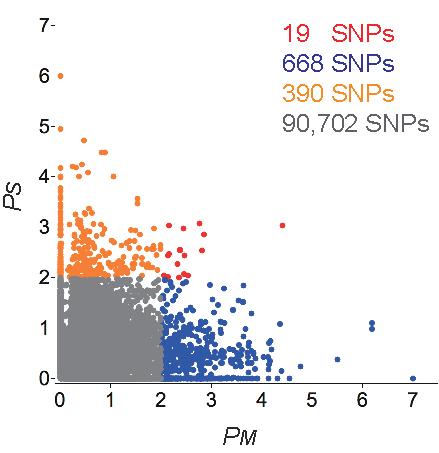
\includegraphics[width=0.4\textwidth]{fig/Fig6}
   \renewcommand{\baselinestretch}{0.9}
   \vspace{-3mm}
   \caption{Scatter plot of $F_{ST}$ $P$-values in Mexico ($P_M$ on $x$-axes) and South America ($P_S$ on $y$-axes).  $P_M$ and $P_S$ are scaled by $-\log_{10}$.  
   \plr{I think you mean these are $-\log_{10} P$-values?}
   \st{yes}
   \plr{It might be nice to label this figure with the numbers in the text, so we can see how many SNPs fall in each category.}
   \st{you mean the numbers of SNPs? How about this?}
   Red, blue, orange and gray dots represents SNPs showing significance in both Mexico and S. America, only in Mexico, only in S. America, respectively (see text for details).
   The number of SNPs in each category is shown in the same color of dots.} 
\vspace{-6mm}
    \label{PvDist}
  \end{center}
\end{figure}
%%%%%%%%%%%%%%%%%%%%%%%%%%%%%%%%%%%%%%%%%% FIGURE
%
%do we know what that clear outlier red SNP is? anything interesting?

\subsection*{Patterns of adaptation}

\subsubsection{Adaptation via mutation versus standing variation}

In order to characterize patterns of adaptation, we first determined whether SNPs showing high differentiation between the lowlands and the highlands arose primarily through new mutations or standing genetic variation.  
We found that these putatively adaptive variants in both Mexico and S. America tended to segregate in lowland populations more often than other SNPs (84.6\% vs. 74.8\% in Mexico, Fisher's exact test (FET) {$P < 10^{-11}$ and 87.3\% vs 81.8\% in South America,  $P< 10^{-3}$).  
\plr{``segregate in'' -- are these percentages of SNPs that are polymorphic (as opposed to fixed for either allele) in the relevant population?}
\st{yes. No fixed allele between Mexico and S. America}
We extended this analysis to standing variation in \emph{parviglumis} by retrieving SNP data from 14 \emph{parviglumis} inbred lines included in the Hapmap v2 data set, using only SNPs with $n\geq10$ \cite[]{Chia_2012_22660545,Hufford_2012_22660546}.  
Again we found that putatively adaptive variants were more likely to be polymorphic in \emph{parviglumis} (81.1\% vs. 72.1\% in Mexico, FET {$P < 10^{-6}$ and 81.2\% vs 72.7\% in South America,  $P< 10^{-4}$).  

\st{add para}
These results suggest that maize adaptation to high altitudes has largely made use of standing genetic variation. 
Recently, examples of adaptation from standing variation have been increased \cite[Reviewed in ][]{Barrett_2008_18006185,Messer_2013_24075201}, and
genome scan studies indicated that soft sweeps are plentiful in Drosophila \cite[]{Garud_2013_ArXiv} and human \cite[]{Turchin_2012_22902787,Peter_2012_23071458}.
Our result is consistent with this view.
In the case of maize, the divergence events occurred very recently \cite[]{Piperno_2006_69,Perry_2006_16511492,Grobman_2012_22307642}.
Thus, it would be unlikely that adaptation via \emph{de novo} mutations frequently occur, which requires a longer waiting time until new beneficial mutations are arisen.
Theoretically, the situation of maize would be consistent with standing variation scenario.
Selection from standing variation are common when scaled mutation rate (the product of effective population size, mutation rate and target size), $\Theta\geq1$ and/or scaled selection coefficient ($Ns$) is enough large \cite[]{Hermisson_2005_15716498}.
Maize should have large $\Theta$ and $Ns$ because the effective population size is relatively large (synonymous nucleotide diversity = 0.014, \cite[\emph{e.g.,} ][]{Tenaillon_2004_15014173,Wright_2005_15919994,Ross-Ibarra_2009_19153259}).

%Sho: please add a sentence or two here on other empirical results on standing var (including the above). We also need a sentence or two here on why we expect this based on theory. I think we drop the domestication comparison
% ST: instead of empirical studies, I added the two nice reviews.  Also added theoretical predictions.

% ST: recombination stuff is moved to subsection "no evidence of parallel adaptation"
%Because linkage disequilibrium in maize decays rapidly \cite[]{Remington_2001_11562485,Tenaillon_2001_11470895} as in our data (Figure~S7), it is plausible that a number of hard sweeps -- strong selection on new mutations -- would be missed by our data, but several lines of evidence suggest to us that this is unlikely.  

%Guys, help here.  My thinking is:
% 1) we see few private SNPs (true? I didn't quite understand your email Sho. what % of SNPs are unique to a population when we include teosinte?
% 2) We do see evidence of selection on other SNPs (at least high Fst), suggesting that even if there are hard sweeps we missed, a substantial amount of selection on standing var appears to have occurred.
% 3) The number of hard sweeps couldn't have been huge or we would see some.
% We need to summarize whether we believe the missed hard sweeps idea is likely or not in a few sentences. Sho, what do you think? Take a stab at it?


\subsubsection{Highland versus lowland adaptation}  

Given the historical spread of maize from an origin in the lowlands, it is tempting to assume that significant population differentiation should be primarily due to an increase in frequency of adaptive alleles in the highlands.
To test this hypothesis, we sought to identify the adaptive allele at each locus using comparisons between Mexico and S. America as well as to \emph{parviglumis} (Text~S1).  Consistent with predictions, we infer that differentiation at 67.5\% (414) and 75.9\% (453) of SNPs in Mexico and S. America is due to adaptation in the highlands, with only 32.5\% (199) and 24.1\% (144) of SNPs inferred to be due to lowland adaptation after excluding the SNPs with ambiguous patterns (probably due to recombination). 
The majority of these SNPs show patterns of haplotype variation (by PHS test) consistent with our inference (Text~S1 and Table~S3).

%
%I think these bar graphs and explanation should go in the supplement. Opinions?
%MBH:I think the edits below improve the narrative, but they gut the results; it makes it easy on the reader that just wants to trust us on the details, but personally I would want more details before I'd buy these results and then I'd be annoyed that I had to dig through the supplement in order to get them.
% ST:         I will make text S1 and Table S3


\subsubsection{Adaptation through introgression}

A marked difference between highland adaptation of maize in Mexico and S. America is the potential for adaptation through introgression from wild relatives.  While maize in Mexico grows in sympatry with both the lowland taxon \textit{parviglumis} and the highland taxon \textit{mexicana}, maize in South America is outside the range of wild \textit{Zea} species.
 \citep{Pyhajarvi2013} recently assessed the potential for local adaptation in \textit{parviglumis} and \textit{mexicana} populations, characterizing differentiation between these subspecies using an Fst-outlier approach.
We observed a significant excess of overlap between our putatively adaptive SNPs in Mexican maize and those identified in the \citep{Pyhajarvi2013} analysis (Table~\ref{tanja}; $P<0.01$ by FET). Similar to that paper, we also find that SNPs with significant $F_{ST}$ $P$-values are enriched in intergenic regions compared to non-significiant SNPs (51.3\% vs. 44.2\%; FET $P < 10^{-8}$). Significant overlap was also observed between significant SNPs in S. America and teosinte ($P<0.01$), but the proportion of SNPs was lower than observed in Mexico.  These data suggest that adaptations in Mexican maize may have been obtained through gene flow with wild relatives.  To more fully explore this hypothesis we evaluated our data in light of introgression identified by \citep{Profford_2013} from \textit{mexicana} into maize in the Mexico highlands.  
The proportion of significant SNPs in introgressed regions in Mexico is significantly higher than found in S. America (FET $P\ll0.001$).
%When focusing on GUs, we identified 99/586 (14.5\%) and 22/466 (4.7\%) GUs of Mexico- and SA-specific significance in introgressed regions (Fisher's exact test, $P<10^{-6}$). 
%Would the genetic unit numbers work in the tanja table? i liek those numbers and think we should keep if possible.
% ST: the number of overlapped SNPs is not big between Tanja's and mine, so it's hard to check GUs.
Outside introgressed regions, the Mexican and S. American populations did not show marked differences in the proportion of significant SNPs (Fisher's exact test, $P>0.7$). These results combined with those from \citep{Profford_2013} suggest that SNPs in introgressed regions have indeed been under selection.  

\subsubsection{No evidence for parallel adaptation}

While maize adaptation in Mexico and S. America are likely distinguished by unique histories of gene flow with wild relatives, the potential remains for parallel adaptation in these two regions.  
SNPs showing significant differentiation between low- and highland populations in both Mexico and S. America are likely candidates for parallel adaptation. 
We identify 56 SNPs with $F_{ST}$ \emph{P}-values in Mexico ($P_M$) and S. America ($P_S$) both $<0.01$.   
This number was significantly larger than the random expectation ($48,370\times 0.01 \times 0.01 \approx 4.8$; $\chi^2$-test, $P\ll0.001$).  Furthermore, the distribution of $P_M$ in the 712 SNPs with $P_S<0.01$ was highly skewed toward zero (Figure~S4A), and a similar tendency was observed in $P_S$ given $P_M<0.01$ (935 SNPs; Figure~S4AB).  Thus, we converted the $P$-values in one population given $P<0.01$ in the other population into $q$-values.  
At a false discovery rate of 0.2 we found 117 SNPs with $P_M<0.01 \cap P_S < 0.0169$ or $P_M<0.0247 \cap P_S < 0.01$, and these SNPs were considered our candidates for parallel adaptation.
We found 959 SNPs showing significant population differentiation only in Mexico ($P_M<0.01 \cap P_S > 0.0169$) and 664 SNPs only in South America  ($P_M>0.0247 \cap P_S < 0.01$).  The scatter plot of $P_M$ and $P_S$ is shown in Figure~\ref{PvDist}.  
For a subset of 67 of the SNPs showing putative evidence of parallel adaptation we also had data from \textit{parviglumis} and were able to infer based on patterns of segregation whether these SNPs were potentially adaptive under lowland or highland conditions (Text~S1).  Surprisingly, SNPs identified as targets of parallel adaptation in Mexico and South America more frequently show segregation patterns consistent with lowland adaptation (62 SNPs) than highland adaptation (5 SNPs). 

In addition to evaluating parallel adaptation at the SNP level, we investigated how often different SNPs in the same gene may have been targeted by selection. To search for this pattern, we define a ``genetic unit" or GU as all SNPs within 10kb of a transcript.  SNPs in an miRNA or second transcript within 10kb of the transcript of interest were excluded.  
We classified SNPs showing significance in Mexico, S. America or in both regions into 1,277 GUs. 
Of these, 95 GUs contained at least one SNP with a pattern of differentiation suggesting parallel adaptation, whereas only 12 GUs contained both Mexico-specific and SA-specific significant SNPs. 
Overall, fewer GUs showed evidence of parallel adaptation than expected by chance (permutation test; $P<10^{-5}$), with more than 700 and 470 GUs showing Mexico-specific and SA-specific significant SNPs, respectively.  
Despite similar phenotypes and environments, we thus see little evidence for parallel adaptation at either the SNP or the gene (GU) level.  

\st{Need your comments!!}
Our result of few parallel adaptation in maize contrasts with data from humans \citep{Tennessen_2011_21698142} showing frequent evidence of selection on the same genes in multiple pairs of tropical and temperate human populations.  
It is common in maize and human that the majority of adaptive variants to high altitudes would be derived from standing variation \cite[]{Tennessen_2011_21698142}.
On the other hand, one difference between these two species is an effective population size.
The effective size of maize (on the oder of $10^5$) is an order of magnitude larger than that in human \cite[]{Takahata_1997_9114074}.
Human would have less potential to possess genetic variants as a source of adaptation, so it could be more likely that the same variants are selected in multiple subpopulations (as long as $s$ is enough large and initial frequency is, for example, $>0.1$).
One the other hand, maize would maintain a larger amount of variants in the ancestral lowland population.
In this case, if genetic variants have almost the same phenotypic effect, the each highland population might pick up one of them randomly.
Or if Mexican and S. American highlands have slightly different climate condition, it is feasible that different variants are selected.
The target size of mutations can also increase the variants for adaptation, but there is no data of this size in maize and human.

Indeed, there are lines of evidence of adaptation from multiple standing variants in maize. % more examples?
One example is \emph{grassy tillers 1} (\emph{gt1}) genes in maize \cite[]{Wills_2013_23825971}.
There are at least two artificially selected mutations on this gene that reduces the number of ears and would be beneficial for the domesticated maize (easy to harvest).
\emph{parviglumis} possesses the two mutations as standing variation with low frequency, and both were spread across maize by selection after domestication.

% ST: LD result is necessary?  Can we say "LD decay looks nice, so genotyping would be nice"?
Because linkage disequilibrium in maize decays rapidly \cite[]{Remington_2001_11562485,Tenaillon_2001_11470895} as in our data (Figure~S5), it is plausible that a number of hard sweeps -- strong selection on new mutations -- would be missed by our data, but several lines of evidence suggest to us that this is unlikely.  


%Points for discussion (add/delete etc.)
%genomic architecture differences? local adaptation uses regulary in teo (cite Tanja)? But what about Fraser (finds same in humans)
% More likely: target size

%this needs to be moved
%CUTME
%While some have hypothesized that pre-adapted highland maize was transported through Central America to the Andes based on analysis of the \emph{Adh2} locus \citep{Freitas_2003_68}, analysis of larger sets of molecular markers suggests \emph{de novo} highland adaptation in South America \citep{Vigouroux_2008_21632329,vanHeerwaarden_2011_21189301}.  Our result of rare parallel adaptation may be consistent with independent origins of highland populations, not gene flow between the two highland populations.
%MBH:Like the discussion above...any way we could include this somewhere?
% ST:  vote in deleting

\subsection*{Comparison to theory}

% # \mutrate computation:
% A <- 500; rho <- 5000; sb <- 10^(-(1:4)); xisq <- 30
% sapply( 10^c(-5,-8), function (mu) mu * (2 * rho * A * sb)/xisq )

For a final point of comparison,
we assessed the degree of parallelism expected under a spatially explicit population genetic model.
We estimate the (maize) population density $\rho$ of the highlands to be around
(0.5 people/km$^2$) $\times$ (0.5 ha field/person) $\times$ ($2\times10^4$ plants per field ha) $=$ 5,000 plants per km$^2$.
The area of the Andean highlands is around $A=500\text{km}^2$, leading to a total population of $A \rho = 2.5 \times 10^6$.
%MBH: This seems like a pretty low planting density
%This should be 14K plants per acre, or ~30-35K per hectare. Good catch Matt!!
%  Moved this up here.  I'm not sure what that 14,000 number was doing in the previous draft.  But, added details behind this calculation.  Should I change anything?
%  Note that 0.5 people/km2 is close to the other number we came up with of "one village per 15km" (which gets 0.4444 people/km2).
Combined with an offspring variance of $\xi^2 = 30$,
we can compute the rate $\mutrate$ at which newly adapted alleles arise in the population.
We observe that even if there is strong selection for an allele at high elevation ($s_b=0.1$),
a single-base mutation with mutation rate $\mu=10^{-8}$ would still take at least 6,000 generations to appear and fix.
On the other hand, a kilobase-sized target with mutation rate $\mu=10^{-5}$
with this selection coefficient would appear and begin to fix in only 6 generations,
while more weakly selected alleles with $s_b$ of $10^{-2}$ or $10^{-3}$ would take hundreds or thousands of generations, respectively.
(Note that the time scales linearly with the selection coefficient: at these values $\Tmut = 1/\mutrate \approx \mu s_b \times 1.6\times 10^5$.)
Therefore, we might expect to see parallel changes of similar effect at the level of genes (e.g.\ disabling mutations),
but would not expect to see adaptive SNPs that arise through independent mutation in the two populations.

% # Tmig computation:
% A <- 500; rho <- 5000; sm <- 10^(-(1:4)); xisq <- 30; sigma <- 1.8
% 1/(sqrt(2*sm)/sigma)
% sapply( 1000*(1:4), function (R) 1 / ( A * rho * ( sqrt(2*sm) / xisq ) * exp(- sqrt(2*sm)*R/sigma ) ) )
% Ne <- (561/10^5)*A*rho 
% Ne  # = 14025
% sapply( 1000*(1:4), function (R) 1 / ( Ne * exp(- sqrt(2*sm)*R/sigma ) ) )

Parallel SNP changes seem unlikely from new mutation; 
what about gene flow between the highlands?
From the demographic model above
we have estimated that $\sigma \approx 1.8$ kilometers per generation,
so with $10^{-1} \ge s_m \ge 10^{-4}$ the distance $\sigma/\sqrt{2s_m}$ over which the frequency of 
a highland-adaptive, lowland-deleterious allele decays into the lowlands
is still short: between 4 and 150 kilometers.
Since the Mexican and Andean highlands are around 4,000 km apart,
the time needed for a rare allele, with selective cost $s_m=10^{-3}$ in the lowlands, to transit between the two highlands
is $\Tmig \approx 5 \times 10^{34}$ generations.
In other words, from these calculations it is almost impossible that an allele that is deleterious at low elevation with $s_m=10^{-3}$ 
would ever transit from the Mexican to the Andean highlands.
If the selection against the allele is even weaker ($s_m=10^{-4}$) it is still expected to take $\Tmig = 1.8 \times 10^8$ generations.
However, shorter distances could be transited by very weakly deleterious alleles --
if the distance between highland patches $R$ is 1,000 km (or if $\sigma$ is four times larger)
then with $s_m=10^{-4}$ the time $\Tmig$ is about 1.6 generations --
so, adaptation by migration is certain in the known timeframe of maize diffusion.
This is strongly dependent on the magnitude of the deleterious selection coefficient: for example,
with $s_m=10^{-3}$, $\Tmig$ is $2.3 \times 10^6$ generations.

This suggests that even when highland-adaptive mutations are weakly deleterious in the lowlands,
gene flow will not result in shared adaptations.
The situation where these are neutral in the lowlands is more difficult to model,
but we can make some informed guesses.
Maize in the Andean highlands, say, would have inherited a lowland-neutral, highland-adapted allele from the Mexican highlands 
if some of the ancestral lineages along which the modern Andean plants have inherited at that locus trace back to the Mexican highlands 
at some point since the appearance of the allele in Mexico.
%MBH:  the previous sentence is pretty convoluted...can this be clarified/simplified?
If the allele is neutral in the lowlands, we can treat this as a neutral process,
using the framework of coalescent theory \citep{wakeley2005coalescent}.
To do this, we need to follow \emph{all} of the $N \approx 2.5 \times 10^6$ lineages backwards; these quickly coalesce to fewer $m$ lineages
in approximately $\sum_{k=m}^N \frac{2N}{\xi^2 k(k+1)} \approx 1.25 \times 10^5/m$ generations,
leaving about 1000 lineages after 100 generations that are spread over a larger area.
The displacement of a lineage after $m$ generations has variance $m \sigma^2$ and is approximately Gaussian.
If we assume that $n$ lineages are independent, and $Z_n$ is the distance to the furthest lineage,
then $\P\{ Z_n / \sqrt{m \sigma^2} \le x /\sqrt{2 \log n} + \sqrt{2 \log n} - (1/2) (\log \log n + \log 4 \pi)/\sqrt{2 \log n} \} \approx \exp( - e^{-x} )$
\citep{berman1964limit}.
With $n=1000$, the typical distance to the furthest displacement after $m=1000$ generations is $\sqrt{2 \sigma^2 m \log n} 212$km;
after $m=6000$ generations it is $\approx 518$km.
In either case, the chance that the maximum is larger than 1,000km after 6,000 generations is well less than $10^{-4}$.
Of course, this is under an equilibrium population model; and maize reached the Andean highlands only around 4,000 years ago.
Nonetheless, this suggests that even highland-adapted allele that are merely neutral in the lowlands
would have difficulty moving between the Mexican and Andean highlands in a few thousand generations.

Based on our spatially explicit population genetic model,
parallel adaptation involving identical nucleotide changes is quite unlikely under either scenarios of independent mutation 
or transit of Central America by undirected (diffusive) sharing of seed.
However, independent mutations could be expected in kilobase-sized targets,
suggesting there might be signal for genes that share adaptive changes.
These conclusions could change if we drastically underestimate the rate of very-long-distance sharing of seed,
e.g.\ if sharing across hundreds of kilometers was common at some point.

